
%(BEGIN_QUESTION)
% Copyright 2006, Tony R. Kuphaldt, released under the Creative Commons Attribution License (v 1.0)
% This means you may do almost anything with this work of mine, so long as you give me proper credit

Electric motors usually rotate at too high of speed to be used directly as valve actuators.  Nearly all electric valve actuators use gear mechanisms to reduce the speed of the electric motor (and multiply its torque).  One of the more popular gear mechanisms for achieving great speed reduction (and torque multiplication) is called the {\it worm gear}:

$$\includegraphics[width=8cm]{i01390x01.eps}$$

The worm wheel's teeth match the pitch of the threads on the worm screw, allowing the two pieces to mesh like gears.  It should be evident from inspection that it takes many, many turns of the work screw to obtain one revolution of the work wheel.  In electric valve actuators, the motor couples to the worm screw and the wheel turns the valve mechanism.

What might not be so evident is how torque on the worm wheel directly translates to linear thrust on the worm screw.  In other words, the more twisting force output by the worm wheel, the greater the straight-line force experienced by the screw:

$$\includegraphics[width=8cm]{i01390x02.eps}$$

If we can find a way to measure this linear thrust on the worm screw, we may infer the torque output by the wheel.  Explain how this could be done in an electric valve actuator mechanism.

\underbar{file i01390}
%(END_QUESTION)





%(BEGIN_ANSWER)

One way to measure worm screw thrust force is with a {\it load cell}.  Another way is to spring-load the screw shaft and use an LVDT or other motion-sensing device to measure displacement.
 
%(END_ANSWER)





%(BEGIN_NOTES)

This is a common way of measuring torque in electric valve actuator mechanisms.

%INDEX% Final Control Elements, valve: electric actuator
%INDEX% Machine, gear (worm)

%(END_NOTES)


